\input{itec625workshopHeader}\section*{Learning outcomes}

By the end of this session, you will know some of Java basics.
In particular, you will be able to design and write simple Java classes.

\section*{Questions}

\begin{questions}

%\question (Problem solving and loops) Write a function (or method) that when passed an integer, returns the number of divisions by two required for the number to reach zero. For example, number of divisions by two required for 19 (or -19) is 5. 
%
%\begin{enumerate}
%\item first time: 19/2 = 9 (not zero, so continue), 
%\item second time: 9/2 = 4 (not zero, so continue), 
%\item third time: 4/2 = 2 (not zero, so continue), 
%\item fourth time: 2/2 = 1 (not zero, so continue), 
%\item fifth time: 1/2 = 0 (stop)
%\end{enumerate}
%
%\begin{solution}
%\begin{lstlisting}
%public static int countDivisonsByTwo(int an) {
%	int count = 0;
%	while(n != 0) {
%		count++;
%		n/=2;
%	}
%	return count;
%}
%\end{lstlisting}
%\end{solution}
%
%\newpage

\question {\bf Import-Export}\\
 
It is important to know how to import Java projects from archive files (.jar/ .zip) and how to export your project(s) into archive files. 

For this exercise, download the file \texttt{classesAndObjectsProgram.zip} from iLearn but \color{red}DO NOT unzip/open it\color{black}.

\begin{enumerate}
\item Click ``File" --> ``Import" --> ``Existing Projects into Workspace" \color{red}\textbf{and NOT "Archive file"}\color{black}.
\item Select option ``Select Archive file" and click on ``Browse"
\item Choose the archive files (``.zip") that contains project(s) you want to open. Please note an archive file may contain multiple projects and click ``ok"
\item Check all projects you want to import
\item Click ``Finish"
\end{enumerate}

You should see a project \texttt{classesAndObjects} if correctly imported.

Next, we'll learn how to export a project.

\begin{enumerate}
\item Click ``File" --> ``Export" --> ``General" --> ``Archive file"
\item Select all projects you want to export in the archive file in the left panel
\item In the ``To archive file" section, choose file path and name
\item Click ``Finish"
\end{enumerate}

Export the project \texttt{classesAndObjects} to an archive file \texttt{exported.zip}.

\newpage
\question Design classes (no implementation) that encapsulate the following real life entities. Add up to three instance variables for each class. Select the three most important attributes if you think a class has more than three attributes. Describe your design in terms of a UML class diagram as shown in the lecture.

\begin{enumerate}
\item \texttt{Person}
\item \texttt{Cylinder}
\item \texttt{Book}
\end{enumerate}

\begin{solution}
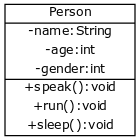
\includegraphics[width=5cm]{Person.png}
\vskip 0.5cm
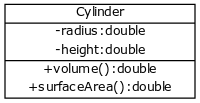
\includegraphics[width=5cm]{Cylinder.png}
\vskip 0.5cm
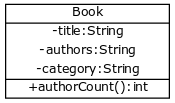
\includegraphics[width=5cm]{Book.png}
\vskip 0.5cm
\end{solution}

\question 

\begin{parts}

\part Consider the following class definition,

\begin{lstlisting}
public class Car {
	public String model;
	public int price;
}
\end{lstlisting}

In a client code (outside the class \texttt{Car}), 

\begin{enumerate}
\item declare and instantiate an object \texttt{myCar} of class \texttt{Car}. 
\item Assign the value \texttt{"Corolla"} to the instance variable \texttt{model} and the value \texttt{21999} to the instance variable \texttt{price} of object \texttt{myCar}.
\end{enumerate}

\begin{solution}
\begin{lstlisting}
Car myCar = new Car();
myCar.model = ``Corolla'';
myCar.price = 21999;
\end{lstlisting}
\end{solution}

\part Consider the following class definition,

\begin{lstlisting}
public class Date {
	public int day, month, year;
}
\end{lstlisting}

In a client code (outside the class \texttt{Date}), 

\begin{enumerate}
\item Declare and instantiate an object \texttt{graduation} of class \texttt{Date}. 
\item Assign values to instance variables of object \texttt{graduation} such that it represents the date 13th April, 2011.
\end{enumerate}

\begin{solution}
\begin{lstlisting}
Date graduation = new Date();
graduation.day = 13;
graduation.month = 4;
graduation.year = 2011;
\end{lstlisting}
\end{solution}

\end{parts}
\newpage

\question 
\begin{parts}

\part Consider the following class definition,

\begin{lstlisting}[frame=single,style=buggy]
public class Time {
	public int hour, minute, second;
}
\end{lstlisting}

Explain why it's a bad idea for the instance variables to be public, by writing a client that is malicious and assigns invalid values to the daa members of \texttt{Time} object.

\begin{solution}
\begin{lstlisting}
Time myTime = new Time();
time.hour = 888;
time.minute = -54;
time.second = -1729;
\end{lstlisting}
\end{solution}

\part Solve the problem of \texttt{public} instance variables in the previous part by first changing visibility of the instance variables of class \texttt{Time} to \texttt{private} and then adding getters and setters. 

\begin{itemize}
\item The setter for \texttt{hour} should constrain the passed value in the range [0, 23]. That is, 

	\begin{itemize}
		\item if the passed value is less than 0, \texttt{hour} should become 0, otherwise,
		\item if the passed value is more than 23, \texttt{hour} should become 23, otherwise,
		\item \texttt{hour} should become the passed value.
	\end{itemize}
\item  Similarly, the setters for \texttt{minute} and \texttt{second} should constrain the passed value in the range [0, 59].
\end{itemize}


\begin{solution}
\begin{lstlisting}
public class Time {
	private int hour, minute, second;

	//setters
	public void setHour(int hour)  {
		if(hour >= 0 && hour <=23)
			this.hour = hour;
		else
			this.hour = 0;
	}

	public void setMinute(int minute)  {
		if(minute >= 0 && minute <=59)
			this.minute = minute;
		else 
			this.minute = 0;
	}

	public void setSecond(int second) {
		if(second >= 0 && second <=59)
			this.second = second;
		else 
			this.second = 0;
	}
	
	//getters
	public int getHour() {
		return hour;
	}

	public int getMinute() {
		return minute;
	}

	public int getSecond() {
		return second;
	}
}
\end{lstlisting}
\end{solution}

\part Declare and instantiate an object \texttt{myTime} of class \texttt{Time} written in the previous part. Assign values to the instance variables such that it represents the time 19:30:45 (half past seven in the evening and another 45 seconds).

\begin{solution}
\begin{lstlisting}
Time myTime = new Time();
myTime.setHour(19);
myTime.setMinute(30);
myTime.setSecond(45);
\end{lstlisting}
\end{solution}

\part Declare and instantiate an object \texttt{yourTime} of class \texttt{Time} written in the previous part. Assign 95 to \texttt{hour}, -78 to minute, and 55 to second. Display all instance variables on the console. What time would \texttt{yourTime} represent?

\begin{solution}
\begin{lstlisting}
Time yourTime = new Time();
yourTime.setHour(95);
yourTime.setMinute(-78);
yourTime.setSecond(55);
System.out.println(yourTime.getHour()); //23
System.out.println(yourTime.getMinute()); //0
System.out.println(yourTime.getSecond()); //55
\end{lstlisting}
\end{solution}

\part List the mistakes (syntactical and logical) in the following constructor for class \texttt{Time} - 

\begin{lstlisting}
public void time(int h) {
	hour = h;
	minute = 0;
	second = 0;
}
\end{lstlisting}

\begin{solution}
\begin{itemize}
\item Constructor has no return type
\item Name of constructor should be \textbf{exactly} the same as the class name.
\item Constructor should use setters to assign values to instance variables.
\end{itemize}

Fixed constructor,

\begin{lstlisting}
public Time(int h) {
	setHour(0);
	setMinute(0);
	setSecond(0);
}
\end{lstlisting}
\end{solution}

\part Add two constructors to class \texttt{Time} with the following requirements:

\begin{itemize}
\item A constructor that is passed three parameters, one for each instance variable.
\item A constructor that is passed two parameters, for \texttt{hour} and \texttt{minute}, and sets \texttt{second} to 0.
\end{itemize}

\begin{solution}
\begin{lstlisting}
public Time(int h, int m, int s) {
	setHour(h);
	setMinute(m);
	setSecond(s);
}

public Time(int h, int m, int s) {
	setHour(h);
	setMinute(m);
	setSecond(0); //default value
}
\end{lstlisting}
\end{solution}

\part Assuming the two constructors have been added to class \texttt{Time} according to previous part. Will the following program run successfully, or result in a compilation error? Explain your answer. Also, if there is a compilation error, what should be done to fix it?

\begin{lstlisting}
Time ourTime = new Time();
\end{lstlisting}

\begin{solution}
It will result in a compilation error, since once parameterized constructors are defined, Java expects us to define the default constructor as well, and the default constructor that Java provides is no longer valid. The solution, therefore, is to add a default constructor.

\begin{lstlisting}
public Time() {
	setHour(0);
	setMinute(0);
	setSecond(0);
}
\end{lstlisting}
\end{solution}
\end{parts}

\vskip 0.5cm

\question {\bf Programming Exercise}\\

\begin{enumerate}
\item Write a class definition for a \texttt{Cylinder}, as represented by its radius and height. It should include,

\begin{enumerate}
\item Correct class header.
\item instance variables with appropriate visibility and data types.
\item Getters
\item Setters, with appropriate validation.
\item Constructors
	\begin{enumerate}
		\item With no parameters. Set each instance variable to 1.
		\item With two parameters, one for each instance variable.
	\end{enumerate}
\item A method \texttt{volume()} that returns the volume of the cylinder. The formula for volume of a cylinder with radius $r$ and height $h$ is $\pi \times r^2 \times h$ (where $r$ is the radius of the circle). The value of $\pi$ in Java is given by \texttt{Math.PI}, and square of a number $n$ is calculated as \texttt{n*n} or \texttt{Math.pow(n,2)}, and \textcolor{red}{NOT \problem{n\^{}2} or \problem{Math.sqr(n)}}.
\end{enumerate}

\item Create a Client \texttt{CylinderClient} that performs the following tasks -

	\begin{enumerate}
	\item Create a \texttt{Cylinder} object \texttt{c1} that has a radius of 2.5 and height of 4.7
	\item Display the volume of \texttt{c1}.
	\item Increase the radius of \texttt{c1} by 2.1
	\item Display the volume of \texttt{c1}.
	\end{enumerate}
	
\end{enumerate}
\begin{solution}
\newpage

Cylinder.java
\begin{lstlisting}
public class Cylinder {
	private double radius, height;
	
	public void setRadius(double r) {
		radius = Math.abs(r);
	}
	
	public void setHeight(double h) {
		height = Math.abs(h);
	}
	
	public double getRadius() {
		return radius;
	}
	
	public double getHeight() {
		return height;
	}
	
	public Cylinder() {
		setRadius(1);
		setHeight(1);
	}
	
	public Cylinder(double r, double h) {
		setRadius(r);
		setHeight(h);
	}
	
	public double volume() {
		return Math.PI * radius * radius * height;
	}		
}
\end{lstlisting}

CylinderClient.java
\begin{lstlisting}
public class CylinderClient {
	public static void main(String[] args) {
		Cylinder c1 = new Cylinder(2.5, 4.7);
		System.out.println(c1.area());
		c1.setRadius(c1.getRadius() + 2);
		System.out.println(c1.area());
	}
}
\end{lstlisting}
\end{solution}

\question \textbf{The \texttt{this} keyword}\\
Consider the following class definition,

\begin{lstlisting}
public class Circle {
	private double radius;
	
	//assume getters, setters, 
	//assume default and parameterized constructors
	
	public boolean equals(Object obj) {
		if(obj instanceof Circle) {
			Circle other = (Circle)obj;
			if(radius == other.radius) {
				return true;
			}
		}
		//in all other cases
		return false;
	}
}
\end{lstlisting}

Further, consider the following client,

\begin{lstlisting}
public class Client {
	public static void main(String[] args) {
		Circle c1 = new Circle(4.5);
		Circle c2 = new Circle(4.8);
		boolean status = c2.equals(c1);
}
\end{lstlisting}

Explain which is the \texttt{this} object and which is the \texttt{obj} object in the context of the method call \texttt{c2.equals(c1)} by drawing a memory diagram.

\begin{solution}
\texttt{this} is a shallow copy of the calling object \texttt{c2} while \texttt{other} is a shallow copy of parameter object \texttt{c1}
\end{solution}

\question \textbf{The \texttt{compareTo} method}\\
Complete the \texttt{compareTo} method in class \texttt{Box} such that it returns,

\begin{itemize}
\item 1, if the calling object has a higher capacity than the parameter object
\item -1, if the calling object has a lower capacity than the parameter object
\item 0, if the calling object has the same capacity as the parameter object
\end{itemize}

\begin{solution}
\begin{lstlisting}
public int compareTo(Box other) {
	if(capacity > other.capacity)
		return 1;
	if(capacity < other.capacity)
		return -1;
	return 0;
}
\end{lstlisting}
\end{solution}
\end{questions}


\end{document}
